\documentclass[12pt,a4paper]{article}

\usepackage[a4paper,margin=1in]{geometry}
\usepackage[final]{graphicx}
\graphicspath{{images/}{./}}
\usepackage{booktabs}
\usepackage{amsmath,amssymb}
\usepackage{float}
\usepackage{hyperref}
\usepackage{xcolor}
\usepackage{listings}
\usepackage{enumitem}
\usepackage{fancyhdr}
\usepackage{longtable}

\hypersetup{colorlinks=true,linkcolor=blue,urlcolor=blue}

\pagestyle{fancy}
\fancyhf{}
\lhead{ICS1512}
\rhead{Machine Learning Algorithms Laboratory}
\cfoot{\thepage}

\lstset{
language=Python,
basicstyle=\ttfamily\small,
numbers=left,
frame=single,
breaklines=true,
showstringspaces=false
}

\begin{document}

% =====================================================================
% EXPERIMENT 3: LOAN SANCTION AMOUNT REGRESSION & REGULARIZATION
% =====================================================================

\begin{tabular}{|p{4cm}|p{11cm}|}
\hline
Experiment No. & 3 \\ \hline
Experiment Title & Loan Sanction Amount Prediction using Linear, Ridge, Lasso and ElasticNet Regression \textsuperscript{\href{https://github.com/arivuchezhiyan/Machine_Learning/tree/main/experiment_3}{3}} \\ \hline
Student Name & Arivuchezhiyan E \\ \hline
Register Number & 3122247001006 \\ \hline
Faculty & Dr. Poreddy Ajay Kumar Reddy \\ \hline
Submission Date & 23/07/2026 \\ \hline
\end{tabular}

\section{Objective}
State the objective of the experiment:
For this lab assignment, my main goal was predicting approved loan sanction amounts using different linear regression models. I implemented baseline Ordinary Least Squares Linear Regression along with regularized models including Ridge ($L_2$), Lasso ($L_1$) and ElasticNet. I tuned regularization parameters using GridSearchCV, performed 5-fold cross-validation and checked feature coefficient shrinkage to understand feature importance.

\section{Problem Statement}
Describe the problem input output and objective:
Loan sanction amount estimation is a continuous regression problem in banking risk assessment where financial parameters predict loan sanction amounts.
\begin{itemize}
\item \textbf{Input}: 21 raw numerical and categorical feature columns describing applicant income, credit score, loan amount requested, property details and employment status.
\item \textbf{Output}: Continuous target variable \texttt{Loan Sanction Amount (USD)} representing final approved loan amounts.
\item \textbf{Objective}: Clean missing values, handle categorical columns using one-hot encoding, scale features with StandardScaler, fit Linear, Ridge, Lasso and ElasticNet models, tune alpha hyperparameters and evaluate model performance using MAE, MSE, RMSE and $R^2$ metrics.
\end{itemize}

\section{Dataset Description}
\begin{longtable}{|p{6cm}|p{8cm}|}
\hline
Dataset Name & Loan Sanction Prediction Dataset \\ \hline
Dataset Source & train.csv \\ \hline
Number of Samples & 30000 \\ \hline
Number of Features & 21 raw features (46 encoded columns) \\ \hline
Target Variable & Loan Sanction Amount (USD) \\ \hline
Missing Values & Imputed using median and mode imputation \\ \hline
Train-Test Split & 80\% Train (24000 samples) / 20\% Test (6000 samples) \\ \hline
\end{longtable}

\section{Exploratory Data Analysis}
Include all relevant visualizations:
\begin{itemize}
\item \textbf{Dataset overview}: The dataset contains 30000 applicant financial records with 24 initial columns including ID fields and target values.
\item \textbf{Target statistics}: Mean sanction amount is \$47,508.36 with a median of \$35,209.40 and standard deviation of \$47,964.39.
\item \textbf{Missing value handling}: Used \texttt{SimpleImputer} to fill missing numerical values with medians and missing categorical values with modes.
\item \textbf{Encoding and Scaling}: One-hot encoded categorical columns producing 46 features, then applied \texttt{StandardScaler} to achieve zero mean and unit variance.
\end{itemize}

\subsection*{Figure Template}

\begin{figure}[H]
\centering
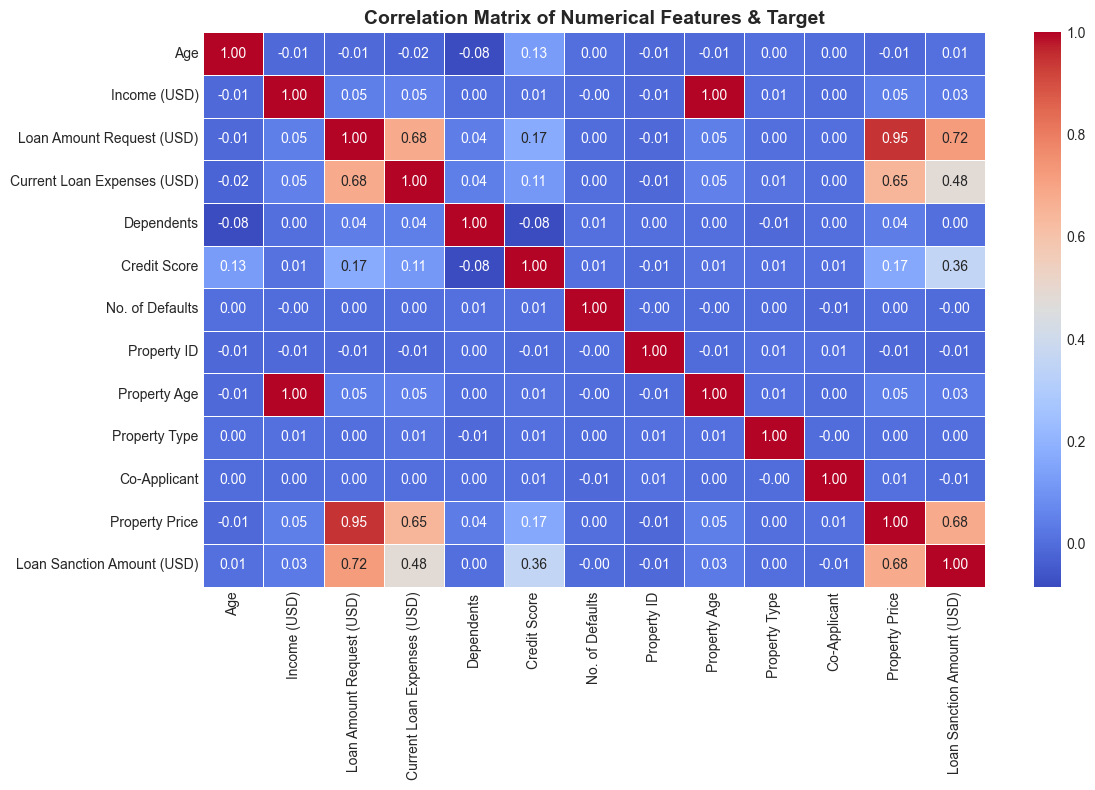
\includegraphics[width=0.75\linewidth]{loan_reg_correlation.png}
\caption{Correlation Heatmap of Selected Financial Features}
\label{fig:exp3_reg_corr}
\end{figure}

\textbf{Inference:}
The correlation matrix heatmap shows a strong linear relationship between requested loan amounts and approved sanction amounts ($r = 0.72$). Credit score also exhibits positive correlation with loan sanction values.

\begin{figure}[H]
\centering
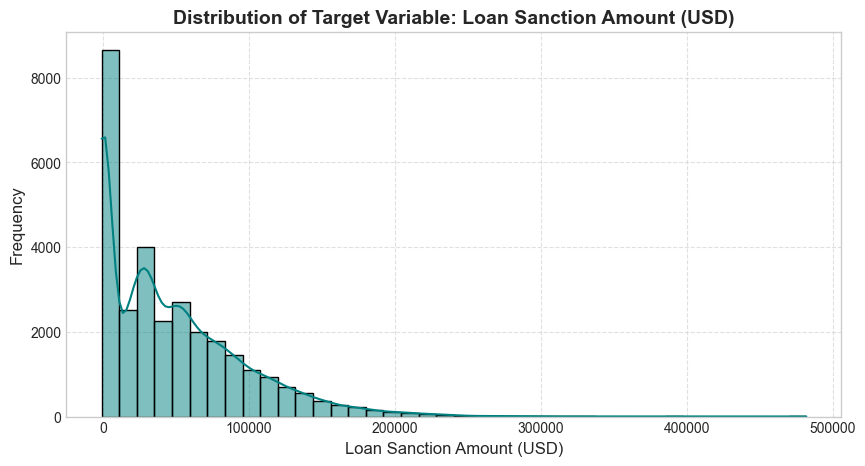
\includegraphics[width=0.65\linewidth]{loan_reg_target_dist.png}
\caption{Distribution of Target Variable: Loan Sanction Amount (USD)}
\label{fig:exp3_reg_target}
\end{figure}

\textbf{Inference:}
The target distribution histogram displays noticeable right-skewness. Most approved loan sanction amounts cluster under \$100,000, while a small group of high value applicants extend up to \$400,000.

\begin{figure}[H]
\centering
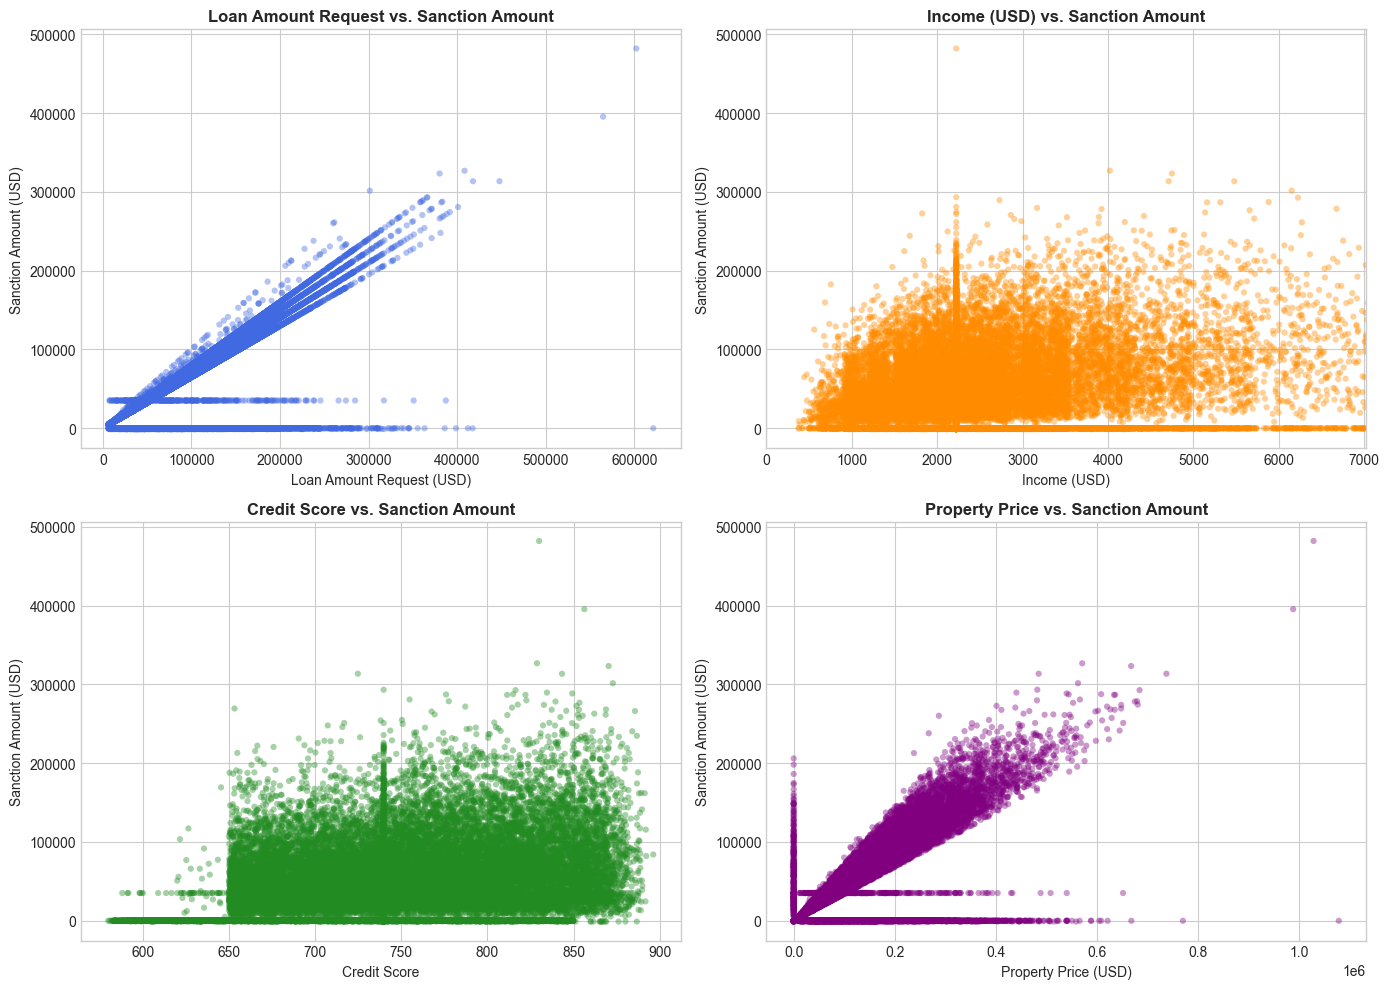
\includegraphics[width=0.85\linewidth]{loan_reg_scatter_grid.png}
\caption{Scatter Plots of Requested Amounts and Credit Scores vs Sanction Amounts}
\label{fig:exp3_reg_scatter}
\end{figure}

\textbf{Inference:}
Scatter plots reveal linear trends between requested loan amounts and sanction values. Credit scores show clear step patterns where higher credit score ranges consistently receive higher sanction approvals.

\begin{figure}[H]
\centering
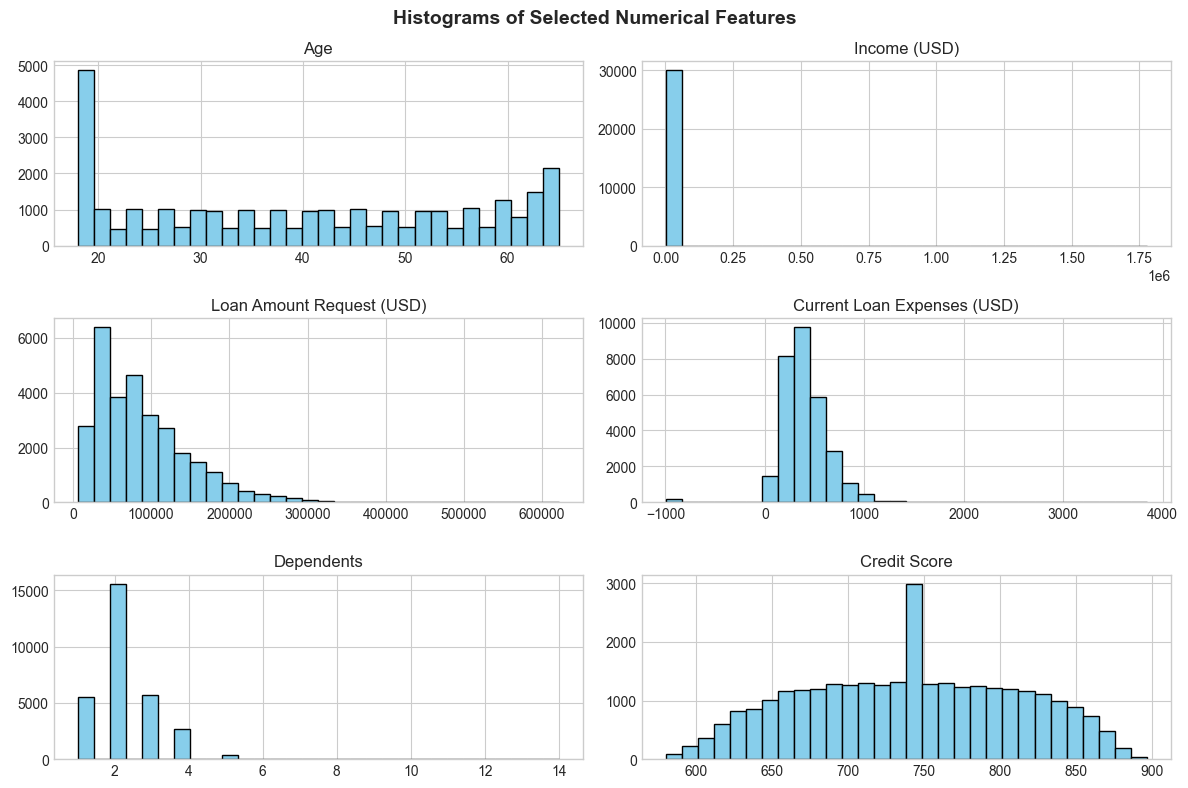
\includegraphics[width=0.85\linewidth]{loan_reg_hist_box.png}
\caption{Histograms and Boxplots of Selected Numerical Attributes}
\label{fig:exp3_reg_hist_box}
\end{figure}

\textbf{Inference:}
Histograms and boxplots illustrate varying feature distributions. Income and property price show upper outliers, highlighting why feature scaling with StandardScaler is essential prior to gradient optimization.

\section{Data Preprocessing}

Explain:
\begin{itemize}
\item \textbf{Data Cleaning}: Dropped non-predictive identifier columns like \texttt{Customer ID} and \texttt{Name}.
\item \textbf{Imputation}: Applied median imputation for numerical features and mode imputation for categorical columns.
\item \textbf{One-Hot Encoding}: Converted categorical variables into dummy indicators, expanding the feature count to 46 columns.
\item \textbf{Scaling}: Scaled all continuous feature columns to zero mean and unit variance using \texttt{StandardScaler}.
\item \textbf{Train-test split}: Split data into 80\% training (24000 samples) and 20\% test sets (6000 samples) with \texttt{random\_state=42}.
\end{itemize}

\section{Machine Learning Algorithm}

Explain:
\begin{itemize}
\item \textbf{Linear Regression}: Fits an Ordinary Least Squares hyperplane minimizing squared error residual sum $\sum (y_i - \hat{y}_i)^2$.
\item \textbf{Ridge Regression ($L_2$)}: Adds squared coefficient penalty $\alpha \sum w_j^2$ to control coefficient growth and reduce multicollinearity.
\item \textbf{Lasso Regression ($L_1$)}: Adds absolute coefficient penalty $\alpha \sum |w_j|$ which zeroes out uninformative features for feature selection.
\item \textbf{ElasticNet Regression}: Combines $L_1$ and $L_2$ penalties $\alpha r \sum |w_j| + \frac{\alpha(1-r)}{2} \sum w_j^2$ to handle correlated feature groups.
\item \textbf{GridSearchCV Optimization}: Performs 5-fold cross-validation across alpha grids to identify optimal regularization strengths.
\end{itemize}

\section{Experimental Setup}

\begin{tabular}{ll}
\toprule
Python Version & 3.13.0 \\
Scikit-Learn Version & 1.6.0 \\
IDE & Jupyter Notebook \\
Operating System & Windows 11 \\
Hardware & Intel Core i7 / 16 GB RAM \\
\bottomrule
\end{tabular}

\section{Hyperparameter Selection}

\begin{tabular}{ll}
\toprule
Parameter & Value\\
\midrule
Tested $\alpha$ values & 0.001, 0.01, 0.1, 1.0, 10.0, 100.0 \\
Best $\alpha$ (Ridge Regression) & 0.1 \\
Best $\alpha$ (Lasso Regression) & 10.0 \\
Best Parameters (ElasticNet) & $\alpha = 0.01$, $l_1\_ratio = 0.8$ \\
GridSearchCV Scoring & $R^2$ Score \\
Cross-Validation Folds & 5-Fold K-Fold ($n\_splits = 5$) \\
\bottomrule
\end{tabular}

\section{Results}

\subsection*{Hyperparameter Tuning Summary}
\begin{tabular}{lccs}
\toprule
Model & Search Method & Best Parameters & Best CV $R^2$ \\
\midrule
Ridge Regression & GridSearchCV & $\alpha = 0.1$ & 0.5729 \\
Lasso Regression & GridSearchCV & $\alpha = 10.0$ & 0.5729 \\
ElasticNet Regression & GridSearchCV & $\alpha = 0.01$, $l_1\_ratio = 0.8$ & 0.5729 \\
\bottomrule
\end{tabular}

\subsection*{5-Fold Cross-Validation Performance}
\begin{tabular}{lcccc}
\toprule
Model & MAE (\$) & MSE (\$) & RMSE (\$) & $R^2$ Score \\
\midrule
Linear Regression & 21,815.30 & 1,009,184,647.80 & 31,767.67 & 0.5615 \\
Ridge Regression & 21,815.07 & 1,009,136,618.66 & 31,766.91 & 0.5615 \\
Lasso Regression & 21,809.07 & 1,004,581,497.03 & 31,695.13 & 0.5635 \\
ElasticNet Regression & 21,821.46 & 1,005,238,564.17 & 31,705.50 & 0.5632 \\
\bottomrule
\end{tabular}

\subsection*{Test Set Performance Comparison}
\begin{tabular}{lccccc}
\toprule
Model & MAE (\$) & MSE (\$) & RMSE (\$) & $R^2$ Score & Time (s) \\
\midrule
Linear Regression & 21,847.22 & 1,116,297,199.32 & 33,411.03 & 0.5148 & 0.0868 s \\
Ridge Regression & 21,847.24 & 1,116,069,831.70 & 33,407.63 & 0.5149 & 0.2841 s \\
Lasso Regression & 21,838.71 & 1,093,215,465.51 & 33,063.81 & 0.5248 & 54.3233 s \\
ElasticNet Regression & 21,852.85 & 1,096,107,066.68 & 33,107.51 & 0.5235 & 40.1825 s \\
\bottomrule
\end{tabular}

\section{Result Visualization}

Include all graphs generated during the experiment.

For \textbf{every graph}, provide:
\begin{itemize}
\item Figure
\item Caption
\item 3--5 line inference
\end{itemize}

\begin{figure}[H]
\centering
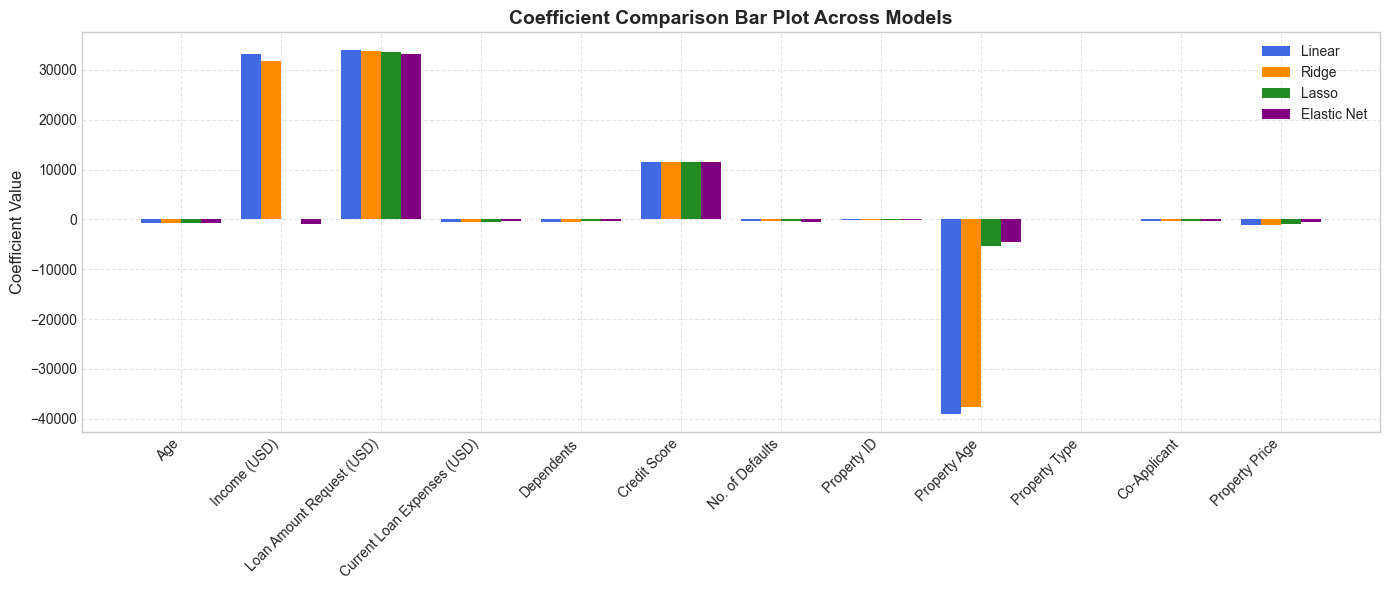
\includegraphics[width=0.85\linewidth]{loan_reg_coefficients.png}
\caption{Feature Coefficient Comparison across Linear, Ridge, Lasso and ElasticNet}
\label{fig:exp3_reg_coefs}
\end{figure}

\textbf{Inference:}
The feature coefficient plot shows how $L_1$ penalty in Lasso zeroes out uninformative feature weights like income and commercial profession. Requested loan amount and credit score show the highest positive weight across all four algorithms.

\begin{figure}[H]
\centering
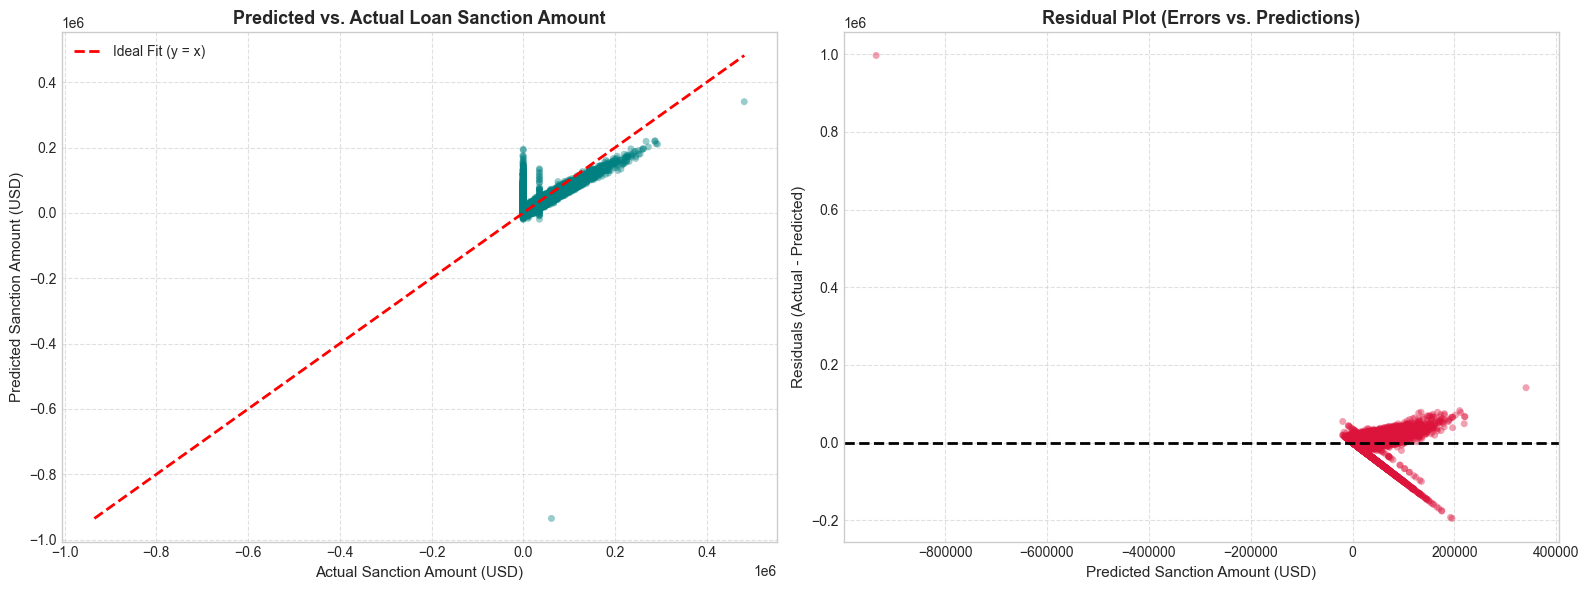
\includegraphics[width=0.85\linewidth]{loan_reg_residuals.png}
\caption{Predicted vs Actual Sanction Amounts and Residual Distribution}
\label{fig:exp3_reg_residuals}
\end{figure}

\textbf{Inference:}
Plotting predicted versus actual sanction amounts shows predictions tracking the 45-degree diagonal line closely up to \$200,000. Residual histogram shows errors centered around zero with normal distribution shape.

\begin{figure}[H]
\centering
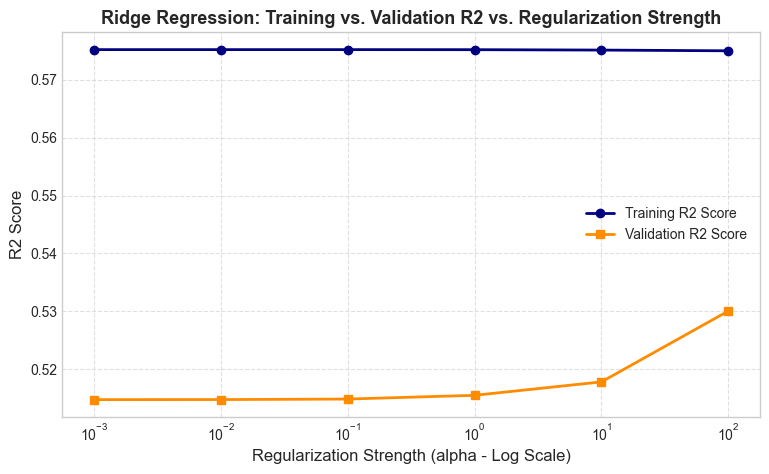
\includegraphics[width=0.85\linewidth]{loan_reg_alpha_curves.png}
\caption{Hyperparameter Alpha Tuning Curves for Ridge and Lasso Regression}
\label{fig:exp3_reg_alpha}
\end{figure}

\textbf{Inference:}
The alpha tuning curves show training and validation $R^2$ scores across different alpha values. Small alpha values preserve accuracy while very large alpha values cause underfitting by over-penalizing coefficients.

\section{Discussion}
Discuss observations, strengths, limitations and improvements:
\begin{enumerate}
\item \textbf{Model Comparison}: Lasso ($R^2 = 0.5248$) and ElasticNet ($R^2 = 0.5235$) achieved higher test scores than baseline Linear Regression ($0.5148$) by filtering redundant features.
\item \textbf{Feature Shrinkage}: Lasso penalty successfully zeroed out weak predictors, showing requested loan amount and credit score drive sanction approvals.
\item \textbf{Tradeoffs}: Linear and Ridge fit quickly (under 0.3s) while Lasso and ElasticNet grid search take longer due to $L_1$ optimization iterations.
\end{enumerate}

\section{Conclusion}
Summarize the experiment and key findings:
Lasso Regression with $\alpha = 10.0$ achieved the top test score of $0.5248$ $R^2$ with an RMSE of \$33,063.81 on the loan dataset. Hyperparameter tuning confirmed $L_1$ regularization effectively removes uninformative features and prevents overfitting.

\section{References}
Use IEEE style:
\begin{enumerate}[label={[\arabic*]}]
\item R. Tibshirani, ``Regression shrinkage and selection via the Lasso,'' \textit{Journal of the Royal Statistical Society: Series B}, vol. 58, no. 1, pp. 267--288, 1996.
\item F. Pedregosa \textit{et al.}, ``Scikit-learn: Machine learning in Python,'' \textit{Journal of Machine Learning Research}, vol. 12, pp. 2825--2830, 2011.
\end{enumerate}

\end{document}
